\documentclass{beamer}
\usetheme{metropolis}

\usepackage[T1]{fontenc}
\usepackage[type1]{libertine}
\renewcommand{\ttdefault}{cmtt}
\usepackage[font=scriptsize]{caption}
\setbeamerfont{footnote}{size=\scriptsize}

\title{Post-processing CDP2 Measurements}
\subtitle{A Quick Overview}
\date{March 2022}

\begin{document}

\frame{\titlepage}

\begin{frame}
    \frametitle{Apply Soft Filter}
    Ensure that all columns have

    \begin{itemize}
        \item DT Bandwidth < 12
        \item Ave Transit Time < 100\footnotemark
    \end{itemize}

    \footnotetext{Maximum allowed transit time is 100 $\mu \mathrm{s}$ (Refer to PADS manuals).}
\end{frame}

\begin{frame}
    \frametitle{Check Dump Spot Monitor (DSM)}
    From PADS Overview manual:

    \begin{quote}
        \small{A channel indicating the amount of focused, unobstructed laser light collected in the dump spot monitor. This channel can indicate overall system health. If the monitor reading goes down when there are no particles present, there may be a problem. (When particles are present, the laser light scatters, which reduces the focused light collected in the dump spot.) It is important to track the trend over a long period of time, for instance over several months, as this channel can change slowly. Overheated lasers or probe windows blocked by fog and/or ice could cause the laser monitor reading to go down even though no particles are present.}
    \end{quote}
\end{frame}

\begin{frame}
    \frametitle{Check Dump Spot Monitor (DSM)}
    Depending on the status of the sensor, one may need to filter out non-spontaneous\footnotemark drops in dump spot monitor (DSM).

    \begin{figure}
        \centering
        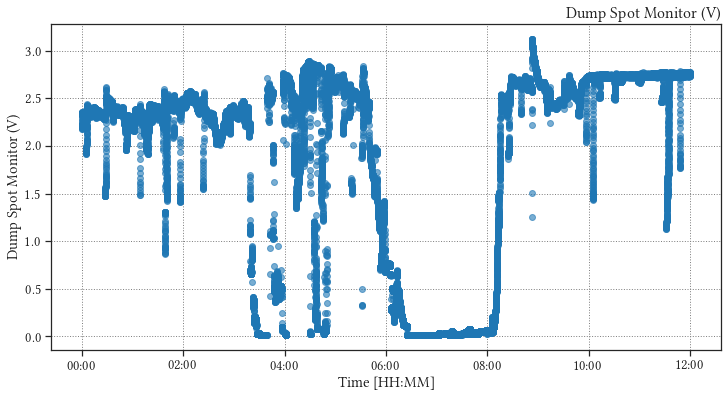
\includegraphics[width=0.8\textwidth]{img/dsm.png}
        \caption{Daily time-series of Dump Spot Monitor [V] on January 15th, 2018.}
    \end{figure}

    \footnotetext{Sudden, short-term drops in DSM due to blockage are expected, but combined with a long-term degradation of the sensor, it is difficult to set a single value for the entire dataset.}
\end{frame}

\begin{frame}
    \frametitle{Adjust with True PAS}
    Because of the discrepancy between the default passing air speed (PAS) and the actual speed of the particles, one needs to estimate the latter based on average transit time:
    \begin{align*}
         & \mathrm{PAS}_\mathrm{LM} / \mathrm{PAS}_\mathrm{True}                                   \\
         & \approx \mathrm{PAS}_\mathrm{LM} / (150 \, [\mu \mathrm{m}] / \tau \, [\mu \mathrm{s}])
    \end{align*}
    where $\tau$ stands for the average transit time measured by CDP2.\\~\

    Multiply all flux-based measurements (e.g. LWC and NC) by the adjustment factor given above.
\end{frame}

\begin{frame}
    \frametitle{Adjust with True PAS}
    \begin{figure}
        \centering
        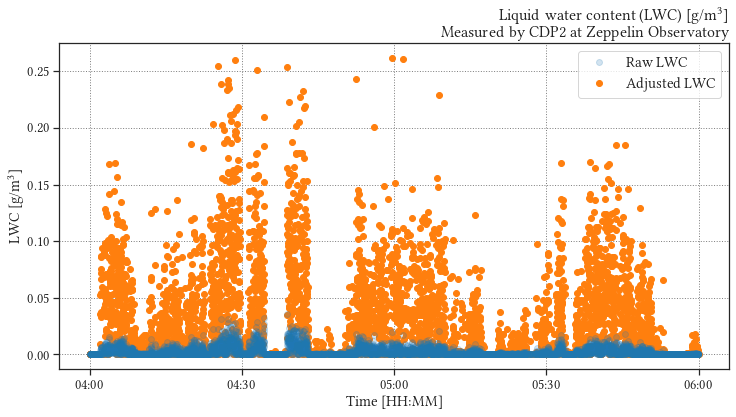
\includegraphics[width=0.8\textwidth]{img/pas.png}
        \caption{Daily time-series of LWC [g/m$^3$] on January 15th, 2018.}
    \end{figure}
\end{frame}

\begin{frame}
    \frametitle{Gassuain Smoothing}
    The raw time-series directly from CDP2 tends to be very noisy. To obtain a more useful (and less error-prone) time-series, one can use the Gaussian kernel:
    \begin{equation*}
        K_\mathrm{Gauss} = \frac{1}{\sigma \sqrt{2 \pi}} \mathrm{e}^{-\frac{x^2}{2 \sigma^2}}
    \end{equation*}
    where $\sigma$ defines the \emph{width} of the kernel. Theoretically, this value represents our prior belief about the uncertainty involved in the observations. We will be using $\sigma = 3$ minutes, since we believe that the flux values do not change rapidly.
\end{frame}

\begin{frame}
    \frametitle{Gassuain Smoothing}
    Given the Gaussian kernel $K_\mathrm{Gauss}$, we can calculate the convolution of the time-series $f(t)$ (LWC in this case) and the Gaussian kernel. That is,
    \begin{equation}
        (f * K_\mathrm{Gauss})(t) \triangleq \int_0^t f(\tau) K_\mathrm{Gauss}(t - \tau) \,\mathrm{d} \tau
    \end{equation}
    which yields a smooth, noise-free time-series.
\end{frame}

\begin{frame}
    \frametitle{Gassuain Smoothing}
    \begin{figure}
        \centering
        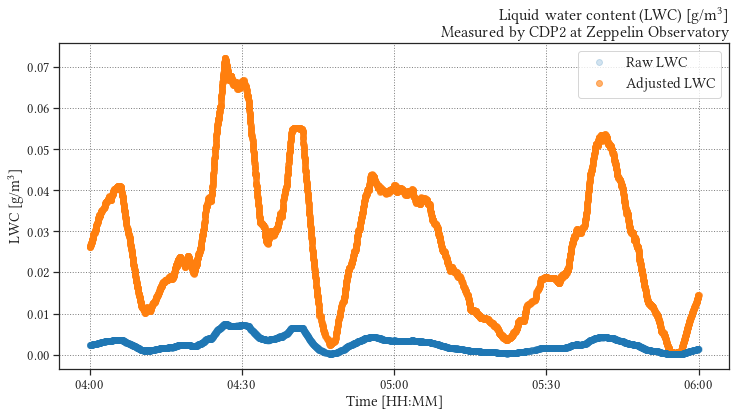
\includegraphics[width=0.8\textwidth]{img/conv.png}
        \caption{Daily time-series of LWC [g/m$^3$] on January 15th, 2018.}
    \end{figure}
\end{frame}

\begin{frame}
    \frametitle{Re-sampling with Sparse GP Model}
    \begin{figure}
        \centering
        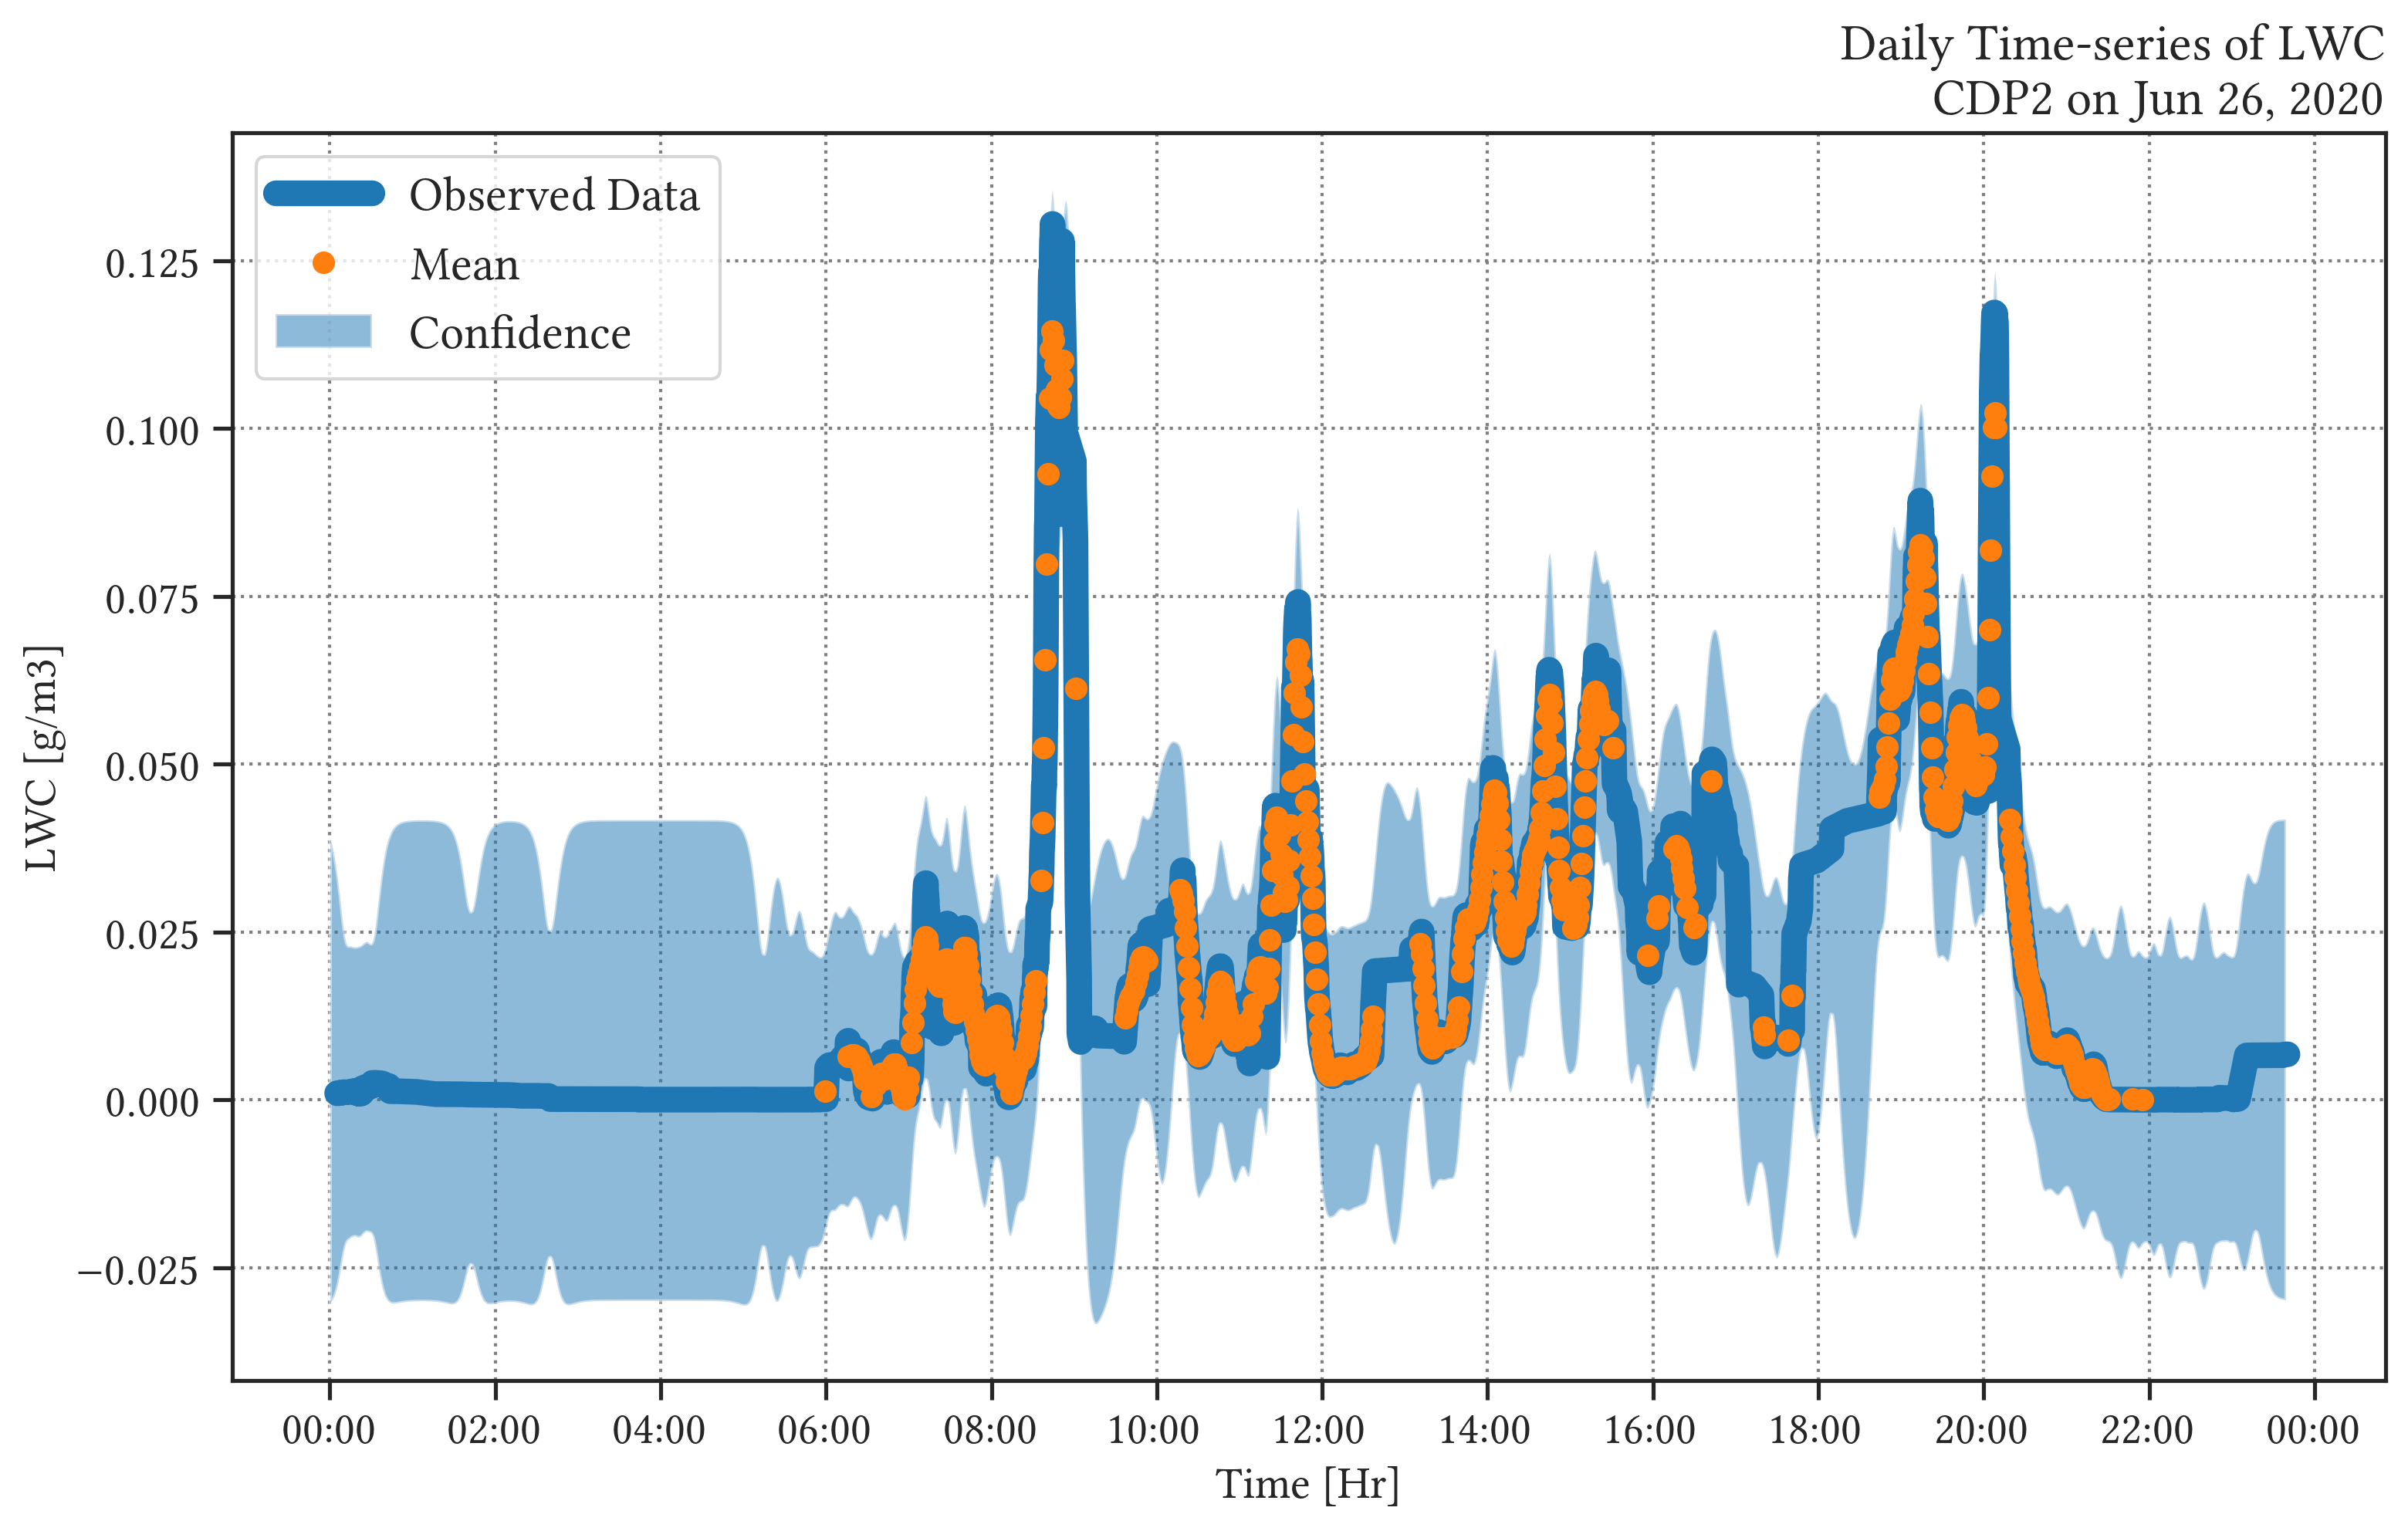
\includegraphics[width=0.8\textwidth]{img/sgp.png}
        \caption{Daily time-series of LWC [g/m$^3$] on January 15th, 2018.}
    \end{figure}

    Resampling allows us to re-define points at which observations are made. In the figure above, the time-series is defined over:
    \begin{equation*}
        T = \{ 0, 30, 60, \dots, 86400 \} \, \mathrm{seconds}.
    \end{equation*}
\end{frame}

\end{document}